\section{WebAssembly Entities}
\label{section:runtime-webassembly-entities}

In the previous section, we discuss the design of the SableWasm WebAssembly
instance object. However, we treat all WebAssembly entities as opaque pointers
without diving into the details during the last section. This section will cover
the implementation of the WebAssembly entities along with the runtime library
builtin functions in SableWasm. Before we start this section, we will first
present the terms used throughout the later part of the thesis. In the rest of
this chapter, we use \texttt{\_\_sable\_instance\_t} to denote the type of the
instance object. Similarly, we use a similar format when discussing WebAssembly
linear memories, indirect tables, and global variables. For example,
\texttt{\_\_sable\_memory\_t} is the type of WebAssembly linear memory in
SableWasm. Finally, we use \texttt{\_\_sable\_function\_t} refer to the function
pointers that point to generated native functions.

\paragraph{Linear Memory}

\begin{figure}
    \centering
    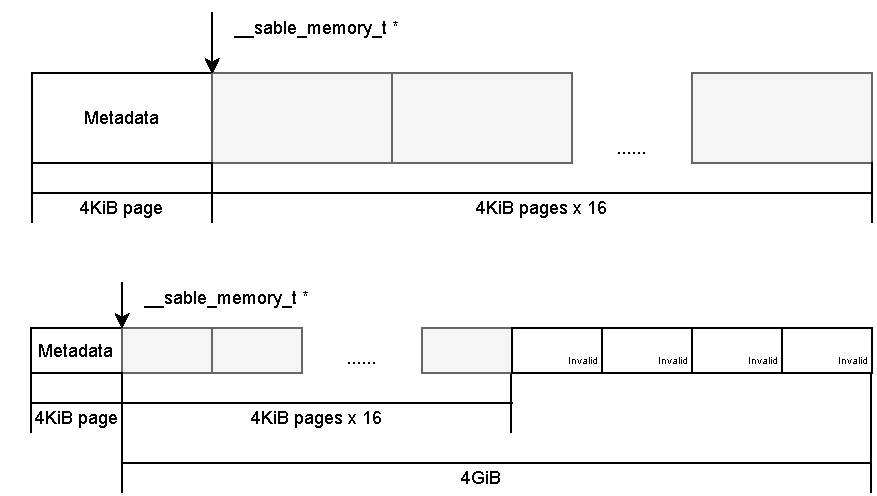
\includegraphics[width=0.85\textwidth]{Images/5.Backend and Runtime/memory}
    \caption{SableWasm WebAssembly linear memory}
    \label{fig:backend-memory}
\end{figure}

SableWasm implements WebAssembly linear memories with mapped memory provided
by the operating system. It also has a fallback implementation that uses
standard \texttt{malloc} and \texttt{free} procedure from the C library for an
operating system that does not support mapped memory. The fallback
implementation is relatively trivial, and we will not discuss it in the thesis.
Here, we will focus on the one that uses mapped memory.
Figure~\ref{fig:backend-memory} illustrates the strategies when mapping
WebAssembly linear memory into native memory. On the top, we have a linear
memory with a size of 1 in WebAssembly page size units, or 64KiB. In the figure,
we assume the native machine has a page size of 4KiB, which is typical for most
hardware architectures. Here's a quick recap on the requirements of WebAssembly
linear memories. First, the program can efficiently random access any location
within the linear memory. Second, at runtime, the module can query
the size of the linear memory. Finally, the program can grow the linear memory
if the runtime system allows it. SableWasm implements linear memories using
a similar trick as the one used for `\texttt{malloc}' functions in many C
standard library implementations. From the generated shared libraries'
perspective, the linear memory object points to the start of a continuous
memory chunk. Hence, memory accesses are efficient and require only one layer
of indirection. First, the generated function will fetch the linear memory base
pointer from the instance object and calculate offsets accordingly.
SableWasm also attaches an extra page that manages the metadata of the linear
memory at the beginning. It contains all the records that the runtime system
needs to work with the linear memory, such as the current size and the upper
bound. Note that the size of the metadata is usually way smaller than the page
size defined by the native machine. Still, SableWasm reserves a whole page for
it, as we want our linear memory start address to be always page-aligned in the
hope of better performance.

\begin{table}[h]
    \centering
    \begin{tabular}{|l|l|}
    \hline
    \textbf{Runtime builtin functions} & \textbf{Description}                              \\ \hline
    \_\_sable\_memory\_size            & Query for the size of the linear memory           \\ \hline
    \_\_sable\_memory\_guard           & Perform boundary check on the linear memory       \\ \hline
    \_\_sable\_memory\_grow            & Attempt to increase the size of the linear memory \\ \hline
\end{tabular}
    \caption{SableWasm runtime builtin functions for linear memory}
    \label{tbl:sablewasm-runtime-memory-api}
\end{table}

SableWasm implements additional functionalities through library functions.
Table~\ref{tbl:sablewasm-runtime-memory-api} illustrates all runtime library
builtin functions provided by SableWasm. \texttt{\_\_sable\_memory\_size}
implements SableWasm's \texttt{MemorySize} instruction. It takes an argument of
a linear memory instance and returns the size of it in WebAssembly page units.
The second runtime builtin function, \texttt{\_\_sable\_memory\_guard}
corresponds to the \texttt{MemoryGuard} instructions in SableWasm. It takes
a linear memory instance and the expected number of bytes ahead as arguments.
Note that the function does not return any values, and this is intentional
by design. SableWasm runtime library utilizes the C++ exception mechanism to
report and handle errors. If the memory access is out-of-bound, the runtime
system will throw an exception. We will come back to this later in this chapter
when discussing the interaction between generated shared libraries and the
host language. Finally, the last runtime builtin function,
\texttt{\_\_sable\_memory\_grow} implements the SableWasm's \texttt{MemoryGrow}
instruction. The instruction follows its counterpart that appeared in the
WebAssembly specification. It takes a linear memory instance and the number of
pages to increase as arguments. If the operation is successful, the function
will yield the new size of the linear memory; otherwise, it returns -1 instead.
SableWasm grows the memory by remapping the memory with the help of the
operating system. On Linux, this usually corresponds to a
\texttt{mremap} operation.

In the above implementation, all linear memory bounds checks are explicit and
program-directed, and thus they are relatively quite expensive. To further
improve the performance, we use a similar technique to that used by many
virtual machine implementations, which utilizes mapped memory access permission
flags. Figure~\ref{fig:backend-memory} illustrates this approach at the bottom.
One may notice that MVP WebAssembly works with 32-bit addressing
\footnote{This is subject to change in the future.
    WebAssembly 64-bit memory addressing:\\
    \url{https://github.com/WebAssembly/memory64}}. Hence, the maximum size of
the linear memory is 4GiB. Thus, SableWasm reserves 4GiB of address when
allocating a linear memory and marks all the pages beyond the current range as
invalid pages. This operation is quite efficient as it only works with the
memory address instead of allocating the memory. In this implementation, any
out-of-bound access will result in a memory segmentation fault. Note that this
strategy does yield better performance but results in a non-recoverable error.
SableWasm provides both implementations, and one can select based on their
needs. In the next chapter, when we compare SableWasm's performance against
several other implementations, we always use the second strategy, as the
recoverable code is not required.

\paragraph{Global}

\begin{figure}
    \centering
    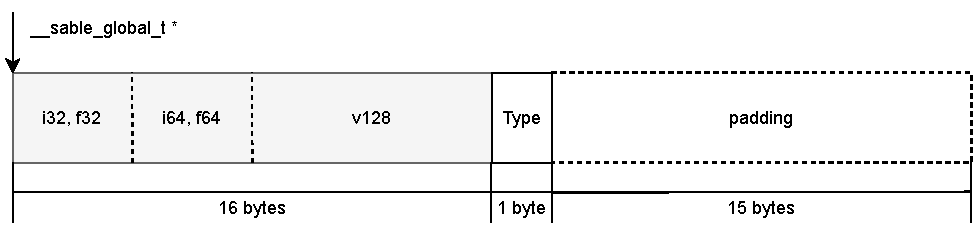
\includegraphics[width=\textwidth]{Images/5.Backend and Runtime/global}
    \caption{SableWasm WebAssembly linear global}
    \label{fig:backend-global}
\end{figure}

Compared to the WebAssembly linear memory implementation, SableWasm's
WebAssembly global variable implementation is relatively straightforward. In
the current version of WebAssembly, global variables can only store primitive
values. Therefore, SableWasm holds the WebAssembly global variable instance as
a union construct of all possible value types, followed by its type's character
encoding. Figure~\ref{fig:backend-global} illustrates SableWasm's implementation
for WebAssembly global variable instances. From the generated shared libraries'
perspective, the global variable access is equivalent to a simple load or store
operation. Note that, in generated shared libraries, we never need to worry
about the mutability of the global variables because the WebAssembly validation
rules ensure that a valid module should never write to a constant global
variable.

\paragraph{Indirect Table}
The last WebAssembly entity implemented in SableWasm is the indirect table, and
it perhaps is the most complex one among all three of them. A quick reminder,
in the instance layout section, we mentioned that we represent the function
instance in SableWasm using function closures that capture its enclosing
context. SableWasm implements the indirect table using a vector of function
closures and their type signatures. The internals of the SableWasm indirect
table is hidden from the generated shared libraries and only communicates to
them via runtime buitlin functions. Table~\ref{tbl:sablewasm-runtime-table-api}
illustrates all the runtime builtin functions provided by SableWasm for
indirect tables.

\begin{table}[h]
    \begin{tabular}{|l|l|}
    \hline
    \textbf{Runtime builtin functions} & \textbf{Description}                                        \\ \hline
    \_\_sable\_table\_guard            & Check if a given index is within the indirect table's range \\ \hline
    \_\_sable\_table\_check            & Check if the entry has specific type                        \\ \hline
    \_\_sable\_table\_context          & Fetch the context pointer of the entry                      \\ \hline
    \_\_sable\_table\_function         & Fetch the function pointer of the entry                     \\ \hline
    \_\_sable\_table\_set              & Write to indirect table                                     \\ \hline
\end{tabular}
    \caption{SableWasm runtime builtin functions for indirect table}
    \label{tbl:sablewasm-runtime-table-api}
\end{table}

\texttt{\_\_sable\_table\_guard} takes the indirect table instance and the
index as arguments. It is quite similar to \texttt{MemoryGuard} instructions,
except that it works with an indirect table. In addition, it also utilizes the
same error handling strategy by throwing an exception in the case where the
index is out-of-bounds. The next runtime builtin function,
\texttt{\_\_sable\_table\_check} implements the runtime type checking for
indirect function calls. It takes a pointer to an indirect table instance,
an index, and a function signature string as the parameter. We use the same
strategy as we have seen in the instance layout section to encode the
expecting type of the function. As in the current SableWasm, the type system is
extremely trivial, there is no complex typing judgment involved, such as
subtyping. Hence, the runtime type checking for indirect function calls is just
a simple string comparison. In the case of type mismatch, the runtime type
checking function also throws an exception. \texttt{\_\_sable\_table\_context}
and \texttt{\_\_sable\_table\_function} are the getter functions provided by
SableWasm. Both of them take an indirect table instance and an index as the
argument. These two functions assume the access is within range, and the
indirect table entry has the expected function type. We will come back to this
later in the chapter when we discuss the patterns used when lowering SableWasm
MIR into LLVM intermediate representations. As their names suggest, the first
function returns the pointer to the context instance object, and the second
function returns the function code address. Finally, the last runtime builtin
function for indirect tables is \texttt{\_\_sable\_table\_set}. Although in MVP
WebAssembly, indirect tables are immutable, the program cannot alter them after
they initialized \footnote{This is subject to change in the future. WebAssembly
    reference types:\\\url{https://github.com/WebAssembly/reference-types}},
the module initialization function still needs the setter function to setup
WebAssembly element segments. The setter function takes an indirect table
instance, an index, a function code address, and its null-terminated type
signature string as the argument. Similar to the getter functions, the setter
function assumes the index is always within range.

The SableWasm runtime library still provides another runtime builtin function
that does not fit into the categories above. SableWasm MIR defines an
\texttt{Unreachable} instruction, which should never reached by any control
flow, and if so, it will signal a runtime panic. In many other languages,
\texttt{Unreachable} maps to a hardware trap instruction, such as \texttt{ud2}
instruction on x86 architecture. However, this behaviour is not acceptable in
SableWasm. \texttt{ud2} generates a non-recoverable hardware invalid instruction
exception, which will eventually lead to the entire system core dump; on
the other hand, SableWasm expects exceptions thrown from generated shared
libraries and should handle them accordingly. Hence, the SableWasm runtime
library provides the \texttt{\_\_sable\_unreachable} function for the SableWasm
MIR \texttt{Unreachable} instruction. We will come back to this with more
details in the following section when discussing the code generation strategy
used when lowering SableWasm MIR into LLVM intermediate representation.